\documentclass{beamer}

\usetheme{Singapore}
\usecolortheme{dove}
\usefonttheme{structurebold}

\usepackage{hyperref}
\usepackage{graphicx}
\usepackage{color}
\usepackage{xcolor}
\usepackage[british]{babel}
%\usepackage[all]{xy}
\usepackage{tikz}
\usepackage{pgfplots}
\usetikzlibrary{positioning}

\title[Plastic Soup recognition]{Detecting Plastic Soup automatically\\ \it \normalsize Using pre-trained Convolutional Neural Networks and Support Vector Machines}
\author[Y. Galama]{Student:\\Ysbrand Galama \\ 10262067 \\[2pc] Supervisor: Thomas Mensink\\}
\institute[UvA]
{
 \includegraphics[width=0.6\textwidth]{images/uva-campus.pdf}
}
\date{29th May 2015}

\begin{document}

	\begin{frame}
	  \titlepage
	\end{frame}

\section{Introduction}
    \begin{frame}{Plastic Soup}
        \begin{itemize}
                \item Large amounts of plastic end up in the world ocean \cite{plastic}
                \item Automate the clean-up process
                \item Develop plastic soup recognition
        \end{itemize}
        \begin{columns}[c]
            \begin{column}{.5\textwidth}
            \end{column}
            \begin{column}{.5\textwidth}
                \includegraphics[width=\textwidth]{images/boat_in_plastic.jpg}\\{\small Figure 1: Boat in plastic soup}
            \end{column}
        \end{columns}
    \end{frame}
 
    \begin{frame}{Current state of the art image techniques I}
        \begin{block}{Convolutional Neural Networks}
            \begin{itemize}
            \item Alexnet implementation to train large amounts of data \cite{alexnet}
            \item Current CNNs very high accuracy \cite{cnn}
            \end{itemize}
        \end{block}
        \includegraphics[width=\textwidth]{images/alexnet2012.png}
    \end{frame}

    \begin{frame}{Current state of the art image techniques II}
        \begin{block}{Support Vector Machine}
            \begin{itemize}
            \item Classification algorithm widely used in CV
            \item Fit a hyperplane in the feature-space
            \item Side of the hyperplane on which a data-point lies is the classifier
            \end{itemize}
        \end{block}
\resizebox{\textwidth}{!}{
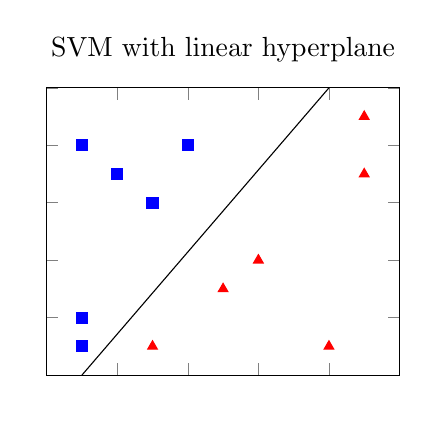
\begin{tikzpicture}
\begin{axis}[
    title={SVM with linear hyperplane},
    width=.5\textwidth,
    xmin=0, xmax=10,
    ymin=0, ymax=10,
    %xtick={0,...,10},
    yticklabels={,,},
    xticklabels={,,},
]
\addplot[
    color=blue,
    mark=square*,
    only marks,
    ]
    coordinates {
    (1,1) (1,2) (1,8) (2,7) (4,8) (3,6)
    };
\addplot[
    color=red,
    mark=triangle*,
    only marks
    ]
    coordinates {
    (3,1) (8,1) (5,3) (6,4) (9,7) (9,9)
    };
\addplot[
    color=black,
    ]
    coordinates{
    (1,0) (8,10)
    };
\end{axis}
\end{tikzpicture}
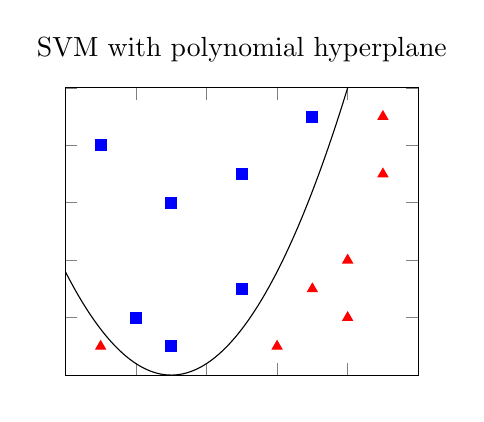
\begin{tikzpicture}
\begin{axis}[
    title={SVM with polynomial hyperplane},
    width=.5\textwidth,
    xmin=0, xmax=10,
    ymin=0, ymax=10,
    %xtick={0,...,10},
    yticklabels={,,},
    xticklabels={,,},
]
\addplot[
    color=blue,
    mark=square*,
    only marks,
    ]
    coordinates {
    (3,1) (2,2) (1,8) (5,7) (7,9) (3,6) (5,3)
    };
\addplot[
    color=red,
    mark=triangle*,
    only marks
    ]
    coordinates {
    (1,1) (6,1) (8,2) (7,3) (8,4) (9,7) (9,9)
    };
\addplot[
    color=black,
    domain=0:10,
    samples=100] (\x,{0.4*(\x-3)^2});
\end{axis}
\end{tikzpicture}
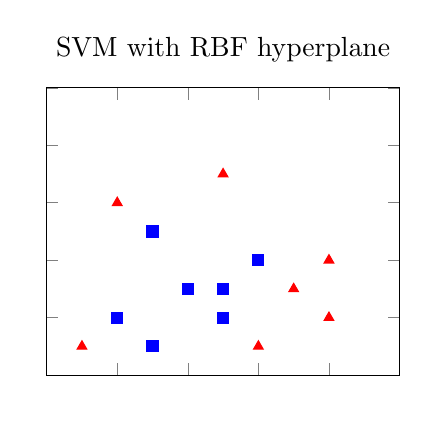
\begin{tikzpicture}
\begin{axis}[
    title={SVM with RBF hyperplane},
    width=.5\textwidth,
    xmin=0, xmax=10,
    ymin=0, ymax=10,
    %xtick={0,...,10},
    yticklabels={,,},
    xticklabels={,,},
]
\addplot[
    color=blue,
    mark=square*,
    only marks,
    ]
    coordinates {
    (3,1) (2,2) (5,2) (4,3) (6,4) (3,5) (5,3)
    };
\addplot[
    color=red,
    mark=triangle*,
    only marks
    ]
    coordinates {
    (1,1) (6,1) (8,2) (7,3) (8,4) (5,7) (2,6)
    };
\draw (axis cs:4,3) circle [black, radius=25];
\end{axis}
\end{tikzpicture}
}
    \end{frame}

    \begin{frame}{Research question}
        \begin{block}{How does a pre-trained CNN in combination with an SVM perform when used for other classifications without being trained on a large amount of domain-specific data?}
        \end{block}
    \end{frame}

\section{Method}
    \begin{frame}{Dataset}
        \begin{columns}[c]
            \begin{column}{.5\textwidth}
                \begin{itemize}
                \item 37165 images from short films
                \item annotated by my hand
                \item 16553 images above and 20612 images below water
                \item 20635 show plastic only
                \item 6972 show animals only
                \item 8502 show both
                \end{itemize}
            \end{column}
            \begin{column}{.4\textwidth}
                \includegraphics[width=\textwidth]{images/10947_01.jpg}\\
                \includegraphics[width=\textwidth]{images/19358_10.jpg}\\
                \includegraphics[width=\textwidth]{images/9077_11.jpg}\\
            \end{column}
        \end{columns}
    \end{frame}

    \begin{frame}{Method and evaluation}
        \begin{block}{Approach}
            \begin{itemize}
            \item Use a pre-trained Convolutional Neural Network as feature extractor
            \item Train an SVM on the second-to-last layer for this specific domain
            \end{itemize}
        \end{block}
        \begin{block}{}
\tikzstyle{image} = [rectangle, draw, fill=blue!20, 
    text width=1.5cm, text centered, minimum height=1cm]
\tikzstyle{cnn} = [rectangle, draw, fill=orange!40,
    text width=2cm, text centered, rounded corners, minimum height=1cm]
\tikzstyle{vector10} = [rectangle, draw, fill=gray!40, 
    text width=1.5cm, text centered, rounded corners, minimum height=1cm]
\tikzstyle{vector1} = [rectangle, draw, fill=gray!20, 
    text width=1.5cm, text centered, rounded corners, minimum height=1cm]
\tikzstyle{svm} = [rectangle, draw, fill=purple!20, 
    text width=1.5cm, text centered, rounded corners, minimum height=1cm]
\tikzstyle{output} = [rectangle, fill=white!0,
    text width=4cm, text centered, rounded corners, minimum height=1cm]
\tikzstyle{labm} = [rectangle, text width=2cm, 
    text centered, minimum height=1cm]
\tikzstyle{line} = [draw, -latex']
\resizebox{\textwidth}{!}{
\begin{tikzpicture}[node distance = 0.5cm, auto]
    \node [image] (a) at (-7,0) {Image};
    \node [labm, above= of a] (at) {Input};
%
    \node [cnn, right=of a] (b) {Caffenet};
    \node [labm, above= of b] (bt) {CNN};
%
    \node [vector10, right=of b] (c) {$10\times4096$};
    \node [labm, above= of c] (ct) {Feature-vector};
%
    \node [vector1, right= of c] (d) {$1\times4096$};
    \node [labm, above= of d] (dt) {Feature-vector};
%
    \node [svm, right= of d] (e) {Animals};
    \node [svm, below= of e] (f) {Plastic};
    \node [labm, above= of e] (et) {SMV};
%
    \node [output, right= of e] (g) {$[0,1]$ showing animals};
    \node [output, right= of f] (h) {$[0,1]$ showing plastic};
    \node [labm, above= of g] (gt) {Output};
%
%
    \path [line] (a) -- (b);
    \path [line] (b) -- (c);
    \path [line] (c) -- (d);
    \path [line] (d) -- (e);
    \path [line] (d) -- (f);
    \path [line] (e) -- (g);
    \path [line] (f) -- (h);
\end{tikzpicture}
}
        \end{block}
    \end{frame}

    \begin{frame}{Method and evaluation}
        \begin{block}{Approach}
            \begin{itemize}
            \item Use a pre-trained Convolutional Neural Network as feature extractor
            \item Train an SVM on the second-to-last layer for this specific domain
            \end{itemize}
        \end{block}
        \begin{block}{Evaluation}
            \begin{itemize}
            \item split dataset in train, validate and test
            \item score the results on the annotated data
            \end{itemize}
            \[
\frac{\#(Outcome_{True}\,and\,Label_{True})+\#(Outcome_{False}\,and\,Label_{False})}{\#tested\,images}
\]
        \end{block}
    \end{frame}

\section{Results}
    \begin{frame}{Results of the pipeline I}
    \begin{block}{}
        \begin{itemize}
        \item linear SVM model works best
        \item $99.9\%$ accuracy on the test-set
        \end{itemize}
    \end{block}
    %\begin{block}{}
\begin{tikzpicture}
%\begin{semilogyaxis}[
\begin{axis}[
    %title={Time and accuracy of different SVM settings with n=14000},
    width=.9\textwidth,
    height=.5\textheight,
    ymin=0, ymax=30000,
    %xmin=0,xmax=21,
    xtick={0,...,21},
    xticklabels={
        %linear,poly:d=2,poly:d=3,poly:d=4,poly:d=5,poly:d=6,poly:d=7,poly:d=8,poly:d=9,rbf:$\gamma$=0.0,rbf:$\gamma$=0.1,rbf:$\gamma$=0.2,rbf:$\gamma$=0.3,rbf:$\gamma$=0.4,rbf:$\gamma$=0.5,rbf:$\gamma$=0.6,rbf:$\gamma$=0.7,rbf:$\gamma$=0.8,rbf:$\gamma$=0.9,rbf:$\gamma$=1.0,
        linear,$\,$,d=2,d=3,d=4,d=5,d=6,d=7,d=8,d=9,$\,$,
        $\gamma$=0.0,$\gamma$=0.1,$\gamma$=0.2,$\gamma$=0.3,$\gamma$=0.4,$\gamma$=0.5,$\gamma$=0.6,
        $\gamma$=0.7,$\gamma$=0.8,$\gamma$=0.9,$\gamma$=1.0,
    },
    x tick label style={rotate=30, anchor=north east, inner sep=0mm},
    xlabel={\hspace{.1cm}${\underbrace{\text{\hspace{3cm}}}\atop\text{polynomial}}$\hspace{0.4cm}${\underbrace{\text{\hspace{4cm}}}\atop\text{rbf}}$},
    xlabel style={at={(0.5,-0.03)}},
    ylabel=Time (sec),
    axis y line*=right,
    enlargelimits=0.05,
    %legend style={at={(0.5,2.2)},anchor=north,legend columns=-1},
    ybar stacked,
    ylabel near ticks,
    scale ticks above exponent={5}
]
\addplot[color=orange!80,fill=orange!80]
    coordinates {
    (0,74.6) (2,1124.4) (3,2068.0) (4,3331.6) (5,4678.5) (6,5198.9) (7,5282.2) (8,5193.3) (9,5083.9) (11,586.3) (12,24560.3) (13,25139.6) (14,25104.7) (15,25389.9) (16,24877.4) (17,26216.1) (18,25266.2) (19,26166.7) (20,18654.6) (21,16250.9)
    };
\addplot[color=purple!70,fill=purple!70]
    coordinates {
    (0,8.4) (2,155.7) (3,277.0) (4,459.8) (5,646.8) (6,696.6) (7,706.6) (8,719.4) (9,714.2) (11,86.2) (12,1067.4) (13,1069.5) (14,1059.1) (15,1052.6) (16,1055.4) (17,1062.9) (18,618.3) (19,1072.2) (20,607.0) (21,399.1)
    };
%\end{semilogyaxis}
\end{axis}
\begin{axis}[
    width=.9\textwidth,
    height=.5\textheight,
    ymin=0,ymax=1,
   % xmin=0,xmax=21,
    x tick label style={color=white},
    ylabel={Accuracy ($\frac{correct}{total}$)},
    axis y line*=left,
    enlargelimits=0.05,
    legend style={at={(0.5,-0.5)},
    anchor=north,legend columns=-1},
    ylabel near ticks,
    ymajorgrids=true,
    xmajorgrids=false,
    grid style=dashed,
]
\addlegendimage{blue, mark=*}
\addlegendimage{only marks, orange!80, mark=square*}
\addlegendimage{only marks, purple!70, mark=square*}
\legend{Accuracy, Train time, Test time}
\addplot[mark=*,blue,jump mark mid]
    coordinates {
    (-1,-10) (0,0.999) (1,-10) (2,0.978) (3,0.964) (4,0.862) (5,0.741) (6,0.606) (7,0.578)
    (8,0.569) (9,0.561) (10,-10) (11,0.991) (12,0.597) (13,0.559) (14,0.554)
    (15,0.554) (16,0.554) (17,0.554) (18,0.554) (19,0.554) (20,0.554)
    (21,0.553) (22,-10)
    };
\end{axis}
\end{tikzpicture}
    %\end{block}
    \end{frame}

    \begin{frame}{Results of the pipeline II}
    \begin{block}{}
        \begin{itemize}
        \item chance of overfitting
        \item using small amounts of train-data
        \item high accuracy with small amounts of train-data
        \end{itemize}
    \end{block}
\resizebox{\textwidth}{!}{
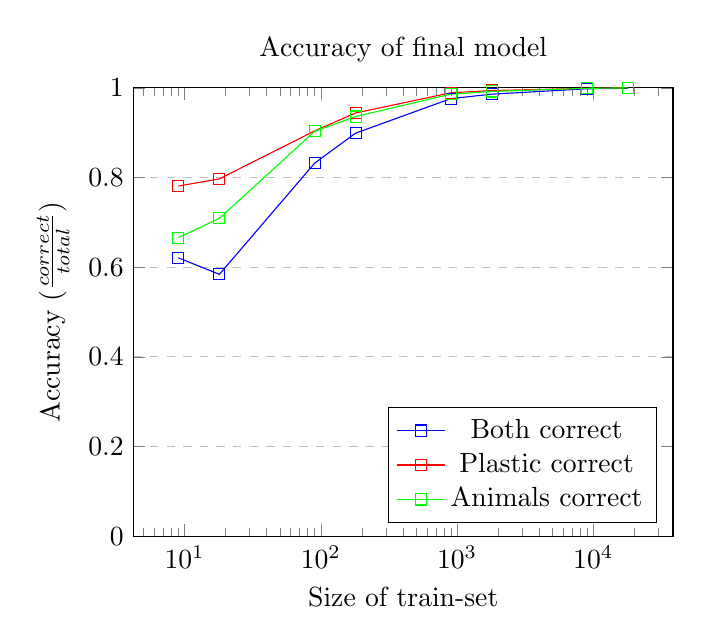
\begin{tikzpicture}
\begin{semilogxaxis}[
    title={Accuracy of final model},
    xlabel={Size of train-set},
    ylabel={Accuracy ($\frac{correct}{total}$)},
    %xmin=0, xmax=18000,
    ymin=0, ymax=1,
    legend pos=south east,
    ymajorgrids=true,
    grid style=dashed,
]
\addplot[
    color=blue,
    mark=square,
    ]
    coordinates {
    (9,0.621)(18,0.584)(90,0.832)(180,0.899)(900,0.976)(1800,0.986)(9000,0.998)(18000,0.999)
    };
    \addlegendentry{Both correct}
\addplot[
    color=red,
    mark=square,
    ]
    coordinates {
    (9,0.781)(18,0.797)(90,0.904)(180,0.944)(900,0.989)(1800,0.994)(9000,0.999)(18000,1.000)
    };
    \addlegendentry{Plastic correct}
\addplot[
    color=green,
    mark=square,
    ]
    coordinates {
    (9,0.666)(18,0.709)(90,0.903)(180,0.936)(900,0.986)(1800,0.992)(9000,0.999)(18000,1.000)
    };
    \addlegendentry{Animals correct}
\end{semilogxaxis}
\end{tikzpicture}
\hspace{.5cm}
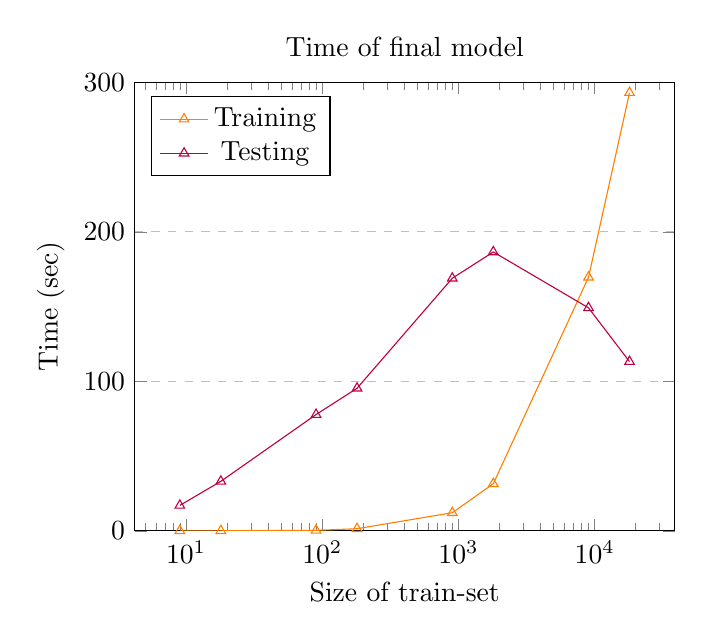
\begin{tikzpicture}
\begin{semilogxaxis}[
    title={Time of final model},
    xlabel={Size of train-set},
    ylabel={Time (sec)},
    %xmin=0, xmax=18000,
    ymin=0, ymax=300,
    legend pos=north west,
    ymajorgrids=true,
    grid style=dashed,
    ]
\addplot[
    color=orange,
    mark=triangle,
    ]
    coordinates {
    (9,0.0)(18,0.0)(90,0.3)(180,1.4)(900,12.1)(1800,31.5)(9000,169.7)(18000,293.2)
    };
    \addlegendentry{Training}
\addplot[
    color=purple,
    mark=triangle,
    ]
    coordinates {
    (9,17.0)(18,33.1)(90,77.8)(180,95.4)(900,169.0)(1800,186.6)(9000,149.2)(18000,113.2)
    };
    \addlegendentry{Testing} 
\end{semilogxaxis}
\end{tikzpicture}
}
    \end{frame}

    \begin{frame}{Localisation of plastic}
    \begin{block}{}
    \begin{itemize}
    \item segment image, run each part through the pipeline
    \item results in heat-map that shows confidence of detecting plastic or animals
    \end{itemize}
    \end{block}
\def\segwidth{.3\textwidth}
\begin{tabular}{ccc}

\includegraphics[keepaspectratio=true,width=\segwidth]{images/segment/6_01__animals__.png} &
\includegraphics[keepaspectratio=true,width=\segwidth]{images/segment/6_01__image__.png} &
\includegraphics[keepaspectratio=true,width=\segwidth]{images/segment/6_01__plastic__.png} \\
\includegraphics[keepaspectratio=true,width=\segwidth]{images/segment/31_11__animals__.png} &
\includegraphics[keepaspectratio=true,width=\segwidth]{images/segment/31_11__image__.png} &
\includegraphics[keepaspectratio=true,width=\segwidth]{images/segment/31_11__plastic__.png}
\end{tabular}
    \end{frame}


\section{Discussion}
    \begin{frame}{Conclusion}
        \begin{block}{Research question}
        How does a pre-trained CNN in combination with an SVM perform when used for other classifications without being trained on a large amount of domain-specific data?
        \end{block}
        \begin{block}{Answer}
        A Linear SVM trained on the second-to-last layer of a pre-trained CNN results in a high accuracy for the task of this project.
        \end{block}
    \end{frame}

    \begin{frame}{Discussion}
        \begin{block}{Improvements for further research}
            \begin{itemize}
            \item construct a better dataset to train and test the CNN and SVM
            \item use more cross-validation on finding parameters
            \item improve localisation of plastic
            \item improve time performance of the pipeline
            \end{itemize}
        \end{block}
        \begin{block}{}
        \Large A step closer to clean up the oceans of Plastic Soup
        \end{block}
    \end{frame}

    \begin{frame}[allowframebreaks]{References}
        \bibliographystyle{abbrv}
        \bibliography{Tex_sources/beamerbib}
    \end{frame}

\end{document}